\documentclass[11pt,twoside,a4paper,openright]{report}
%%%%%%%%%%%%%%%%%%%%%%%%%%%%%%%%%%%%%%%%%%%%%%%%
% Language, Encoding and Fonts
% http://en.wikibooks.org/wiki/LaTeX/Internationalization
%%%%%%%%%%%%%%%%%%%%%%%%%%%%%%%%%%%%%%%%%%%%%%%%
% Select encoding of your inputs. Depends on
% your operating system and its default input
% encoding. Typically, you should use
%   Linux  : utf8 (most modern Linux distributions)
%            latin1 
%   Windows: ansinew
%            latin1 (works in most cases)
%   Mac    : applemac
% Notice that you can manually change the input
% encoding of your files by selecting "save as"
% an select the desired input encoding. 
\usepackage[utf8]{inputenc}
% Make latex understand and use the typographic
% rules of the language used in the document.
\usepackage[english]{babel}
% Use the palatino font
\usepackage[sc]{mathpazo}
\linespread{1.05}         % Palatino needs more leading (space between lines)
% Choose the font encoding
\usepackage[T1]{fontenc}

%%%%%%%%%%%%%%%%%%%%%%%%%%%%%%%%%%%%%%%%%%%%%%%%
% Graphics and Tables
% http://en.wikibooks.org/wiki/LaTeX/Importing_Graphics
% http://en.wikibooks.org/wiki/LaTeX/Tables
% http://en.wikibooks.org/wiki/LaTeX/Colors
%%%%%%%%%%%%%%%%%%%%%%%%%%%%%%%%%%%%%%%%%%%%%%%%
% load a colour package
\usepackage{xcolor}
\definecolor{aaublue}{RGB}{33,26,82}% dark blue
% The standard graphics inclusion package
\usepackage{graphicx}
% Set up how figure and table captions are displayed
\usepackage{caption}
\captionsetup{%
  font=footnotesize,% set font size to footnotesize
  labelfont=bf % bold label (e.g., Figure 3.2) font
}
% Make the standard latex tables look so much better
\usepackage{array,booktabs}
% Enable the use of frames around, e.g., theorems
% The framed package is used in the example environment
\usepackage{framed}

% Adds support for full page background picture
\usepackage[contents={},color=gray]{background}
%\usepackage[contents=draft,color=gray]{background}

%%%%%%%%%%%%%%%%%%%%%%%%%%%%%%%%%%%%%%%%%%%%%%%%
% Mathematics
% http://en.wikibooks.org/wiki/LaTeX/Mathematics
%%%%%%%%%%%%%%%%%%%%%%%%%%%%%%%%%%%%%%%%%%%%%%%%
% Defines new environments such as equation,
% align and split 
\usepackage{amsmath}
% Adds new math symbols
\usepackage{amssymb}
% Use theorems in your document
% The ntheorem package is also used for the example environment
% When using thmmarks, amsmath must be an option as well. Otherwise \eqref doesn't work anymore.
\usepackage[framed,amsmath,thmmarks]{ntheorem}

%%%%%%%%%%%%%%%%%%%%%%%%%%%%%%%%%%%%%%%%%%%%%%%%
% Page Layout
% http://en.wikibooks.org/wiki/LaTeX/Page_Layout
%%%%%%%%%%%%%%%%%%%%%%%%%%%%%%%%%%%%%%%%%%%%%%%%
% Change margins, papersize, etc of the document
\usepackage[
  inner=28mm,% left margin on an odd page
  outer=41mm,% right margin on an odd page
  ]{geometry}
% Modify how \chapter, \section, etc. look
% The titlesec package is very configureable
\usepackage{titlesec}
\titleformat{\chapter}[display]{\normalfont\huge\bfseries}{\chaptertitlename\ \thechapter}{20pt}{\Huge}
\titleformat*{\section}{\normalfont\Large\bfseries}
\titleformat*{\subsection}{\normalfont\large\bfseries}
\titleformat*{\subsubsection}{\normalfont\normalsize\bfseries}
%\titleformat*{\paragraph}{\normalfont\normalsize\bfseries}
%\titleformat*{\subparagraph}{\normalfont\normalsize\bfseries}

% Clear empty pages between chapters
\let\origdoublepage\cleardoublepage
\newcommand{\clearemptydoublepage}{%
  \clearpage
  {\pagestyle{empty}\origdoublepage}%
}
\let\cleardoublepage\clearemptydoublepage

% Change the headers and footers
\usepackage{fancyhdr}
\pagestyle{fancy}
\fancyhf{} %delete everything
\renewcommand{\headrulewidth}{0pt} %remove the horizontal line in the header
\fancyhead[RE]{\small\nouppercase\leftmark} %even page - chapter title
\fancyhead[LO]{\small\nouppercase\rightmark} %uneven page - section title
\fancyhead[LE,RO]{\thepage} %page number on all pages
% Do not stretch the content of a page. Instead,
% insert white space at the bottom of the page
\raggedbottom
% Enable arithmetics with length. Useful when
% typesetting the layout.
\usepackage{calc}

%%%%%%%%%%%%%%%%%%%%%%%%%%%%%%%%%%%%%%%%%%%%%%%%
% Bibliography
% http://en.wikibooks.org/wiki/LaTeX/Bibliography_Management
%%%%%%%%%%%%%%%%%%%%%%%%%%%%%%%%%%%%%%%%%%%%%%%%
\usepackage[backend=bibtex,
  bibencoding=utf8,
  style=numeric-comp
  ]{biblatex}
\addbibresource{bib/mybib}

%%%%%%%%%%%%%%%%%%%%%%%%%%%%%%%%%%%%%%%%%%%%%%%%
% Misc
%%%%%%%%%%%%%%%%%%%%%%%%%%%%%%%%%%%%%%%%%%%%%%%%
% Hide the ugly red borders around clickable hyperlinks/references
\usepackage[hidelinks]{hyperref}
% Add bibliography and index to the table of
% contents
\usepackage[nottoc]{tocbibind}
% Add the command \pageref{LastPage} which refers to the
% page number of the last page
\usepackage{lastpage}
% Add todo notes in the margin of the document
\usepackage[
%  disable, %turn off todonotes
  colorinlistoftodos, %enable a coloured square in the list of todos
  textwidth=\marginparwidth, %set the width of the todonotes
  textsize=scriptsize, %size of the text in the todonotes
  ]{todonotes}

%%%%%%%%%%%%%%%%%%%%%%%%%%%%%%%%%%%%%%%%%%%%%%%%
% Hyperlinks
% http://en.wikibooks.org/wiki/LaTeX/Hyperlinks
%%%%%%%%%%%%%%%%%%%%%%%%%%%%%%%%%%%%%%%%%%%%%%%%
% Enable hyperlinks and insert info into the pdf
% file. Hypperref should be loaded as one of the 
% last packages
\usepackage{hyperref}
\hypersetup{%
	pdfpagelabels=true,%
	plainpages=false,%
	pdfauthor={Author(s)},%
	pdftitle={Title},%
	pdfsubject={Subject},%
	bookmarksnumbered=true,%
	colorlinks=false,%
	citecolor=black,%
	filecolor=black,%
	linkcolor=black,% you should probably change this to black before printing
	urlcolor=black,%
	pdfstartview=FitH%
}

%%%%%%%%%%%%%%%%%%%%%%%%%%%%%%%%%%%%%%%%%%%%%%%%
% Listings (Code Snippets)
% https://en.wikibooks.org/wiki/LaTeX/Source_Code_Listings
%%%%%%%%%%%%%%%%%%%%%%%%%%%%%%%%%%%%%%%%%%%%%%%%
\usepackage{listings}
\usepackage{color}

\renewcommand{\lstlistingname}{Code Snippet} % Listing -> Code Snippet
\definecolor{lighter-gray}{RGB}{240,240,240}

\lstset{
  backgroundcolor=\color{lighter-gray},
  extendedchars=true,
  basicstyle=\footnotesize\ttfamily,
  showstringspaces=false,
  showspaces=false,
  numbers=left,
  tabsize=4,
  breaklines=true,
  showtabs=false,
  captionpos=b,
  numberstyle=\footnotesize,
  numbersep=5pt
}

% Define C# as a snippet language.
\usepackage{courier}

\definecolor{Green}{rgb}{0, 0.3, 0}
\definecolor{DarkCyan}{rgb}{0, 0.545, 0.545}
\definecolor{Navy}{rgb}{0, 0, 0.5}
\definecolor{Teal}{rgb}{0, 0.5, 0.5}
\definecolor{DarkGray}{gray}{0.66}
\definecolor{Olive}{rgb}{0.5, 0.5, 0}
\definecolor{Pink}{rgb}{1.0, 0.75, 0.8}
\definecolor{DeepPink}{rgb}{1, 0.08, 0.58}
\definecolor{Brown}{rgb}{0.65, 0.165, 0.165}
\definecolor{DarkViolet}{rgb}{0.58, 0, 0.83}
\definecolor{SaddleBrown}{rgb}{0.55, 0.27, 0.07}
\definecolor{Orange}{rgb}{0.9, 0.427, 0}
\lstdefinelanguage{CSharp}{
  morecomment = [l]{//}, 
  morecomment = [l]{///},
  morecomment = [s]{/*}{*/},
  morestring=[b]", 
  morestring=[b]',
  basicstyle=\footnotesize\ttfamily,
  commentstyle=\color{Green}\textit,
  stringstyle=\color{Orange},
  sensitive = true,
  morekeywords=[1]{this, base},
  keywordstyle=[1]\bfseries\color{Navy},
  morekeywords=[2]{as, is, new, sizeof, typeof, true, false, stackalloc},
  keywordstyle=[2]\color{Navy}\bfseries,
  morekeywords=[3]{else, if, switch, case, default,
  do, for, foreach, while, in},
  keywordstyle=[3]\bfseries\color{Navy} ,
  morekeywords=[4]{break, continue, goto, return,
  yield, partial, global, where},
  keywordstyle=[4]\bfseries\color{Navy},
  morekeywords=[5]{try, throw, catch, finally},
  keywordstyle=[5]\color{Navy}\bfseries,
  morekeywords=[6]{checked, unchecked},
  keywordstyle=[6]\color{Navy}\bfseries,
  morekeywords=[7]{fixed, unsafe},
  keywordstyle=[7]\bfseries\color{Navy},
  morekeywords=[8]{bool, byte, sbyte, char, short, ushort, int, uint, long, ulong, float,
  double, decimal, enum, struct},
  keywordstyle=[8]\bfseries\color{Navy},
  morekeywords=[9]{class, interface, delegate, object, string,
  void},
  keywordstyle=[9]\bfseries\color{Navy},
  morekeywords=[10]{explicit, implicit, operator},
  keywordstyle=[10]\bfseries\color{Navy},
  morekeywords=[11]{params, ref, out},
  keywordstyle=[11]\bfseries\color{Navy},
  morekeywords=[12]{private, protected, internal, public},
  keywordstyle=[12]\bfseries\color{Navy},
  morekeywords=[13]{abstract, const, event, var, override, virtual, volatile, extern, readonly, sealed, static},
  keywordstyle=[13]\bfseries\color{Navy},
  morekeywords=[14]{namespace, using},
  keywordstyle=[14]\bfseries\color{Navy},
  morekeywords=[15]{lock},
  keywordstyle=[15]\bfseries\color{Navy},
  morekeywords=[16]{get, set, add, remove},
  keywordstyle=[16]\bfseries\color{Navy},
  morekeywords=[17]{null, value},
  keywordstyle=[17]\bfseries\color{Navy},
}
\newcommand{\userStory}[3]{
  \begin{center}
    \begin{tabular}{|p{0.8\textwidth}|} 
     \hline
     \textbf{USER STORY}\\
     As \textit{#1}\\
     I want to be able to #2\\
     so I #3.\\ [0.5ex] 
     \hline
    \end{tabular}
    \end{center}  
    }
\usepackage{multirow}

\titleformat*{\subsubsection}{\large\bfseries}
\titleformat*{\subsection}{\Large\bfseries}
\titleformat*{\section}{\LARGE\bfseries}% package inclusion and set up of the document
% see, e.g., http://en.wikibooks.org/wiki/LaTeX/Formatting#Hyphenation
% for more information on word hyphenation
\hyphenation{ex-am-ple hy-phen-a-tion short}
\hyphenation{long la-tex}
% 
% see, e.g., http://en.wikibooks.org/wiki/LaTeX/Customizing_LaTeX#New_commands
% for more information on how to create macros

%%%%%%%%%%%%%%%%%%%%%%%%%%%%%%%%%%%%%%%%%%%%%%%%
% Macros for the titlepage
%%%%%%%%%%%%%%%%%%%%%%%%%%%%%%%%%%%%%%%%%%%%%%%%
%Creates the aau titlepage
\newcommand{\aautitlepage}[3]{%
  {
    %set up various length
    \ifx\titlepageleftcolumnwidth\undefined
      \newlength{\titlepageleftcolumnwidth}
      \newlength{\titlepagerightcolumnwidth}
    \fi
    \setlength{\titlepageleftcolumnwidth}{0.5\textwidth-\tabcolsep}
    \setlength{\titlepagerightcolumnwidth}{\textwidth-2\tabcolsep-\titlepageleftcolumnwidth}
    %create title page
    \thispagestyle{empty}
    \noindent%
    \begin{tabular}{@{}ll@{}}
      \parbox{\titlepageleftcolumnwidth}{
        \iflanguage{danish}{%
          
\includegraphics[width=\titlepageleftcolumnwidth]{AAUgraphics/aau_logo_da}
        }{%
          
\includegraphics[width=\titlepageleftcolumnwidth]{AAUgraphics/aau_logo_en}
        }
      } &
      \parbox{\titlepagerightcolumnwidth}{\raggedleft\sf\small
        #2
      }\bigskip\\
       #1 &
      \parbox[t]{\titlepagerightcolumnwidth}{%
      \textbf{Abstract:}\bigskip\par
        \fbox{\parbox{\titlepagerightcolumnwidth-2\fboxsep-2\fboxrule}{%
          #3
        }}
      }\\
    \end{tabular}
    \vfill
    \iflanguage{danish}{%
      \noindent{\footnotesize\emph{Rapportens indhold er frit tilgængeligt, men offentliggørelse (med kildeangivelse) må kun ske efter aftale med forfatterne.}}
    }{%
      \noindent{\footnotesize\emph{The content of this report is freely available, but publication (with reference) may only be pursued due to agreement with the author.}}
    }
    \clearpage
  }
}

%Create english project info
\newcommand{\englishprojectinfo}[8]{%
  \parbox[t]{\titlepageleftcolumnwidth}{
    \textbf{Title:}\\ #1\bigskip\par
    \textbf{Theme:}\\ #2\bigskip\par
    \textbf{Project Period:}\\ #3\bigskip\par
    \textbf{Project Group:}\\ #4\bigskip\par
    \textbf{Participant(s):}\\ #5\bigskip\par
    \textbf{Supervisor(s):}\\ #6\bigskip\par
    \textbf{Copies:} #7\bigskip\par
    \textbf{Page Numbers:} \pageref{LastPage}\bigskip\par
    \textbf{Date of Completion:}\\ #8
  }
}

%Create danish project info
\newcommand{\danishprojectinfo}[8]{%
  \parbox[t]{\titlepageleftcolumnwidth}{
    \textbf{Titel:}\\ #1\bigskip\par
    \textbf{Tema:}\\ #2\bigskip\par
    \textbf{Projektperiode:}\\ #3\bigskip\par
    \textbf{Projektgruppe:}\\ #4\bigskip\par
    \textbf{Deltager(e):}\\ #5\bigskip\par
    \textbf{Vejleder(e):}\\ #6\bigskip\par
    \textbf{Oplagstal:} #7\bigskip\par
    \textbf{Sidetal:} \pageref{LastPage}\bigskip\par
    \textbf{Afleveringsdato:}\\ #8
  }
}

%%%%%%%%%%%%%%%%%%%%%%%%%%%%%%%%%%%%%%%%%%%%%%%%
% An example environment
%%%%%%%%%%%%%%%%%%%%%%%%%%%%%%%%%%%%%%%%%%%%%%%%
\theoremheaderfont{\normalfont\bfseries}
\theorembodyfont{\normalfont}
\theoremstyle{break}
\def\theoremframecommand{{\color{gray!50}\vrule width 5pt \hspace{5pt}}}
\newshadedtheorem{exa}{Example}[chapter]
\newenvironment{example}[1]{%
		\begin{exa}[#1]
}{%
		\end{exa}
}

\newcommand{\knox}{Knox}
\newcommand{\postgres}{PostgreSQL}% my new macros

\begin{document}
%frontmatter
\pagestyle{empty} %disable headers and footers
\pagenumbering{roman} %use roman page numbering in the frontmatter
%\pdfbookmark[0]{Front page}{label:frontpage}%

\begin{titlepage}
\newgeometry{top=0cm,bottom=1.2cm,right=0cm,left=0cm}

  \backgroundsetup{
   scale=1.1,
   angle=0,
   opacity=1.0,  %% adjust
   contents={\includegraphics[width=\paperwidth,height=\paperheight]{AAUgraphics/aau_waves}}
    }
		
  \begin{center} %%please do not change the height or width of the frontpage image
    \centerline{
\includegraphics[totalheight=0.5\paperwidth,width=1\paperwidth]{AAUgraphics/frontpageImage}}% 
  \end{center}
	
	\vspace*{-0.96cm}
  {\noindent\color{aaublue}\fboxsep0pt\colorbox{white}{\begin{tabular}{@{}p{\paperwidth}@{}}
    \centerline{
    \begin{minipage}{0.85\textwidth}
        \bigskip
				\bigskip
        \centering
        \Huge{\textbf{
A simple explanation of how our Universe was formed% insert your title here
        }}
    \end{minipage}
    }
		
	\centerline{
	\begin{minipage}{0.9\textwidth}
        \bigskip
        \centering
        \Large{
Development of a predictive model% insert your subtitle here
        }
    \end{minipage}
    }
			
	\centerline{
	\begin{minipage}{0.9\textwidth}
        \bigskip
        \centering
        {\Large
Anders Andersen, Alfred Alfredsen, Anne Annesen% insert names separated by comma
        }
    \end{minipage}
    }
			
    \centerline{
    \begin{minipage}{0.9\textwidth}
        \bigskip
        \centering
        {\large
Energy Technology, TEPE4-1005, \the\year-06% insert name of study, group number, year-month
        } 
    \end{minipage}
    }
			
    \centerline{
    \begin{minipage}{0.9\textwidth}
        \bigskip
        \centering
%% Comment this section if you are not doing Bachelor or Master Project   
        {\Large
Master's Project
      %Bachelor Project
        }
        \smallskip
    \end{minipage}
    }
			
  \end{tabular}}}

  \vfill
  \begin{figure}[!b]
	\centering
    
\includegraphics[width=0.2\paperwidth]{AAUgraphics/aau_logo_circle_en}% comment this line in for English version
    %
\includegraphics[width=0.2\paperwidth]{AAUgraphics/aau_logo_circle_da} %comment this line in for Danish version
  \end{figure}
\end{titlepage}
\restoregeometry
\pdfbookmark[0]{Front page}{label:frontpage}%
\begin{titlepage}
\vspace*{\fill}
    \backgroundsetup{
    scale=1.1,
    angle=0,
    opacity=1.0,  %% adjust
    contents={\includegraphics[width=\paperwidth,height=\paperheight]{AAUgraphics/aau_waves}}
    }
  \addtolength{\hoffset}{0.5\evensidemargin-0.5\oddsidemargin} %set equal margins on the frontpage - remove this line if you want default margins
  \noindent%
  {\color{white}\fboxsep0pt\colorbox{aaublue}{\begin{tabular}{@{}p{\textwidth}@{}}
    \begin{center}
    \Huge{\textbf{
      A study on the Universe% insert your title here
    }}
    \end{center}
    \begin{center}
      \Large{
        Development of a predictive model% insert your subtitle here
      }
    \end{center}
    \vspace{0.2cm}
   \begin{center}
    {\Large
      Anders Andersen, Alfred Alfredsen, Anne Annesen% insert names separated by comma
    }\\
    \vspace{0.2cm}
    {\large
      Energy Technology, TEPE4-1005, 2018-06% insert name of study, group number, year-month
    }
   \end{center}
   \vspace{0.2cm}
%% Comment this section in if you are doing Bachelor or Master Project   
   \begin{center}
    {\Large
      Master's Project
      %Bachelor Project
    }
   \end{center}
  \end{tabular}}}
  \vfill
  \begin{center}
    
\includegraphics[width=0.2\paperwidth]{AAUgraphics/aau_logo_circle_en}% comment this line in for English version
    %
\includegraphics[width=0.2\paperwidth]{AAUgraphics/aau_logo_circle_da} %comment this line in for Danish version
  \end{center}
\end{titlepage}
\clearpage

\thispagestyle{empty}
{\small
\strut\vfill % push the content to the bottom of the page
\noindent Copyright \copyright{} Aalborg University 2015\par
\vspace{0.2cm}
\noindent Here you can write something about which tools and software you have used for typesetting the document, running simulations and creating figures. If you do not know what to write, either leave this page blank or have a look at the colophon in some of your books.\todo{Add a colophon}
}
\clearpage


\pdfbookmark[0]{English title page}{label:titlepage_en}
\aautitlepage{%
  \englishprojectinfo{
    Placeholder Title %title
  }{%
    Scientific Theme %theme
  }{%
    Fall Semester 2021 %project period
  }{%
    cs-21-sw-5-19 % project group
  }{%
    %list of group members
    Christian Bager Bach Houmann\\
    Daniel Overvad Nykjær\\
    Ivik Lau Dalgas Hostrup\\
    Marco Klaustrup Justesen\\
    Patrick Frostholm Østergaard\\
    Rasmus Høyer Hansen
  }{%
    %list of supervisors
    Christian Aebeloe
  }{%
    1 % number of printed copies
  }{%
    \today % date of completion
  }%
}{%department and address
  \textbf{Computer Science}\\
  Aalborg University\\
  \href{http://www.aau.dk}{http://www.aau.dk}
}{% the abstract
Knox (Knowledge Engineering Toolbox) is a continuous pipeline project involving several project groups working in scrum-inspired environment.
This report documents the work of the third layer of the pipeline, responsible for database and server management.
For the first half of the project, the groups collaborated on developing a search engine.
Here we designed and implemented database structures in the relational database management system PostgreSQL.
This report then documents this design and the implementation of the required API endpoints to access it using HTTP.
For the second half of the project, the groups began development of features based on knowledge graphs.
 Here we supported the other groups by implementing a data storage for the used RDF data. 
}

% \cleardoublepage
% {\selectlanguage{danish}
% \pdfbookmark[0]{Danish title page}{label:titlepage_da}
% \aautitlepage{%
%   \danishprojectinfo{
%     Rapportens titel %title
%   }{%
%     Semestertema %theme
%   }{%
%     Efterårssemestret 2010 %project period
%   }{%
%     XXX % project group
%   }{%
%     %list of group members
%     Forfatter 1\\ 
%     Forfatter 2\\
%     Forfatter 3
%   }{%
%     %list of supervisors
%     Vejleder 1\\
%     Vejleder 2
%   }{%
%     1 % number of printed copies
%   }{%
%     \today % date of completion
%   }%
% }{%department and address
%   \textbf{Elektronik og IT}\\
%   Aalborg Universitet\\
%   \href{http://www.aau.dk}{http://www.aau.dk}
% }{% the abstract
%   Her er resuméet
% }}
% 
\cleardoublepage
\pdfbookmark[0]{Contents}{label:contents}
\pagestyle{fancy} %enable headers and footers again
\tableofcontents
\listoftodos
\chapter*{Preface\markboth{Preface}{Preface}}\label{ch:preface}
\addcontentsline{toc}{chapter}{Preface}
Group cs-21-sw-5-19 will hereby referred to as \textit{our group}, \textit{our}, or \textit{we} for the purpose of this document.
This report is a documentation of the work done by our group in the course of the semester.

We would like to extend our thanks to our supervisor \textit{Christian} for the support and guidance that we received throughout the semester.

\vspace{\baselineskip}\hfill Aalborg University, \today
\vfill\noindent


\begin{minipage}[b]{0.45\textwidth}
 \centering
 \rule{\textwidth}{0.5pt}\\
 Christian Bager Bach Houmann\\
 {\footnotesize <chouma19@student.aau.dk>}
\end{minipage}

\hfill
\begin{minipage}[b]{0.45\textwidth}
 \centering
 \rule{\textwidth}{0.5pt}\\
  Daniel Overvad Nykjær\\
 {\footnotesize <dnykja18@student.aau.dk>}
\end{minipage}

\begin{minipage}[b]{0.45\textwidth}
 \centering
 \rule{\textwidth}{0.5pt}
  Ivik Lau Dalgas Hostrup\\
 {\footnotesize <ihostr16@student.aau.dk>}
\end{minipage}

\hfill
\begin{minipage}[b]{0.45\textwidth}
 \centering
 \rule{\textwidth}{0.5pt}
  Marco Klaustrup Justesen\\
 {\footnotesize <mkju19@student.aau.dk>}
\end{minipage}

\begin{minipage}[b]{0.45\textwidth}
 \centering
 \rule{\textwidth}{0.5pt}
  Patrick Frostholm Østergaard\\
 {\footnotesize <pfas19@student.aau.dk>}
\end{minipage}

\hfill
\begin{minipage}[b]{0.45\textwidth}
 \centering
 \rule{\textwidth}{0.5pt}
  Rasmus Høyer Hansen\\
 {\footnotesize <mkju19@student.aau.dk>}
\end{minipage}
\cleardoublepage
%mainmatter
\pagenumbering{arabic} %use arabic page numbering in the mainmatter

% ! Place your sections here !
\chapter{Problem Formulation}
\section{Semester Context}
This semester is thematically based on students learning how to collaborate as teams on a complex project.

To accommodate this, students work in interdependent teams on separate parts of a complex project. 
Each team has a specific role, and should, to some degree, provide support to teams that they are collaborating with.
To this, students are taught certain software process models, and are expected to use them in their work.
This is supposed to emulate the environment of an actual software project.

We are part of the Knox multi-project. In the next section, we will describe Knox and our role in more detail.
% However, it is important to note that Knox is developed using Agile software development practices.
% This is also the process model that we will be using in this semester.
% 
% The choice to use Agile software development practices is not a technical decision, but rather a choice of a process model that is suitable for the type of work that we are doing.
% We find the benefits of an Agile approach superior to other models, considering the scope, details, and requirements for the project.
% To specify, we will be dealing with many of unknowns, which means that the flexibility of an agile approach will be beneficial.



% A case could be made for the waterfall model, in that we have a certain deadline for delivering a report, and the phases of writing the report (and the deadline) are known beforehand. 
% However, the contents of the report is what is important, and that will only become better by 1. following and learning from the designated process, and 2. doing good work, which the agile approach — in our estimation — would help us do.
% The work that we will do was, when we started the project, largely unknown.
% 
% Similarly, a case could be made for the integration and configuration model.
% We could do much of our assigned task by integrating and configuring various 3rd party components and systems. 
% However, we would like to learn as much as we can. 
% As such, the approach of using the work of others is not ideal — even if you learn a few things by implementing it.

\section{KnoxLayer}
The knowledge engineering toolkit or Knox is a project which goal is to provide a flexible toolkit whose components can be combined to solve bigger problems. Here the long-term vision for Knox is to provide access to chatbots and personal assistants that can provide a proven answer to the users' questions through the usage of knowledge extraction, natural language processing, fact-checking, explainable ai. 
The overall goal for the 2nd iteration of Knox is to complete a search engine with the provided components from the 1st iteration. Furthermore, a shared interface for the front-end and back-end and an advancement of its components is expected. 


The Knox project itself is currently split into a 4-layered pipeline structure. The first layers of the pipeline is the Pre-processing layer which takes image files as input. Here the goal is to convert the image files into text files using optical image recognition. 


Once the first layer has completed its objective the files are then sent to the next stage of the pipeline being the Knowledge layer. The main task here is to extract as much data as possible from the files generated by the previous layer using natural language processing. Here the data is extracted in the form of RDF triples which consists of a subject, an object, and the predicate connecting them. 


Next up the 3rd layer also known as the data layer handles the data management and integration across the board. This layer is responsible for managing all the data extracted during the different stages of the pipeline and making sure it is available for the next stages when needed. 


The final stage of the pipeline is the functionality layer. This layer handles all the functionalities that are available for the end-user. These functionalities cover fact-checking and providing an explanation for the given prediction.


With an overview of the current state of the overall main objectives of the project  established a more in-depth look at the current state of the data layer is now needed to continue the development of the layer. 




% \chapter{Introduction}\label{ch:introduction}
Here is the introduction. The next chapter is chapter~\ref{ch:ch2label}.


a new paragraph


\section{Examples}
You can also have examples in your document such as in example~\ref{ex:simple_example}.
\begin{example}{An Example of an Example}
  \label{ex:simple_example}
  Here is an example with some math
  \begin{equation}
    0 = \exp(i\pi)+1\ .
  \end{equation}
  You can adjust the colour and the line width in the {\tt macros.tex} file.
\end{example}

\section{How Does Sections, Subsections, and Subsections Look?}
Well, like this
\subsection{This is a Subsection}
and this
\subsubsection{This is a Subsubsection}
and this.

\paragraph{A Paragraph}
You can also use paragraph titles which look like this.

\subparagraph{A Subparagraph} Moreover, you can also use subparagraph titles which look like this\todo{Is it possible to add a subsubparagraph?}. They have a small indentation as opposed to the paragraph titles.

\todo[inline,color=green]{I think that a summary of this exciting chapter should be added.}

% \chapter{Chapter 2 name}\label{ch:ch2label}
Here is chapter 2. If you want to leearn \todo{I think this word is mispelled} more about \LaTeXe{}, have a look at\cite{Madsen2010}, \cite{Oetiker2010} and\cite{Mittelbach2005}.
\missingfigure{We need a figure right here!}


% \chapter{Conclusion}\label{ch:conclusion}
The code that we overtook from last year for the search engine was incomplete and did not work.
We therefore implemented the database from scratch using C\# and the Entity Framework Core.
Our first attempt at this went well as is fulfilled the requirements provided by the Product Owner. 
This was verified through an end to end test where all layers participated.
However, despite this, the design had a major flaw in terms of excessive memory consumption. 
Fortunately, near the end of the project, we were able to allocate time to a redesign which addressed this problem.
We were unable to create a BCNF design on time though, and we therefore believe that the database group next year should prioritize this.

The solution from last year used to store RDF data was deemed problematic.
It required periodic restarts in order to move the data from in memory into persistent disk storage.
Therefore, a large effort was made into building a new system for handling the \knox{} RDF data storage needs. 
Here, Virtuoso was deemed as an appropriate framework since it lived up to the requirements provided from the other layers. 

Both databases were tested using Postman to ensure that the endpoints work as intended.
A few unit tests were also written for JSON validator, however the database functionality itself remains largely untested as we cannot, and should not, test a framework.

The main purpose of this semester project was to obtain knowledge and experience in analysis, design, implementation and evaluation of complex software systems in a large development environment \cite{AAULearningGoals5thSemester}.
Due to different understandings of agile and scrum, however, conflicts and problems arose intermittently.
Several committees were created whose purpose was to dictate specific guidelines or be responsible for certain aspects.
Some groups disagreed with the decisions made by those committees, and as there was no concrete project lead, nothing could truly be enforced. 
The lack of a project lead also meant that suggestions and complaints from groups resulted in little to no changes.


Another goal of this semester was to learn proper version control and module encapsulation, however this idea fell short due to the complete lack of security for the \knox{} repositories. 
Any group could simply force code into other groups' repositories, which caused time-consuming conflicts to occur.
In addition, other groups would suddenly request new features that needed to be implemented urgently.


Consequently, due to the aforementioned structural and management issues, it was difficult to follow a concrete sprint planning structure.


Ultimately, we feel as though the concept of \knox{} is good, however the execution was unfortunate. 
While we did learn a lot, the rough nature of the project and its conflicts have resulted in division among students. 
Internally, the structure of \knox{} resulted in a productive workflow for the group as a whole. 
We believe that the positive workflow we experienced internally may also flourish across group collaboration in future projects when these issues have been addressed.
% If you do not write the report in English, translating the bibliography title to, e.g., Danish, should not be done here. Instead, you should change the main language in the preamble (look for the line \usepackage[danish,english]{babel} and change the order/delete the 'english' option). See more in the babel package documentation.
\printbibliography[heading=bibintoc, title=Bibliography]
\label{bib:mybiblio}
\appendix
\chapter{Appendix A name}\label{ch:appAlabel}
Here is the first appendix

\chapter{Data access models}\label{AppDataAccess}
% % JsonSchemaModel
\begin{figure}[H]
    \centering
    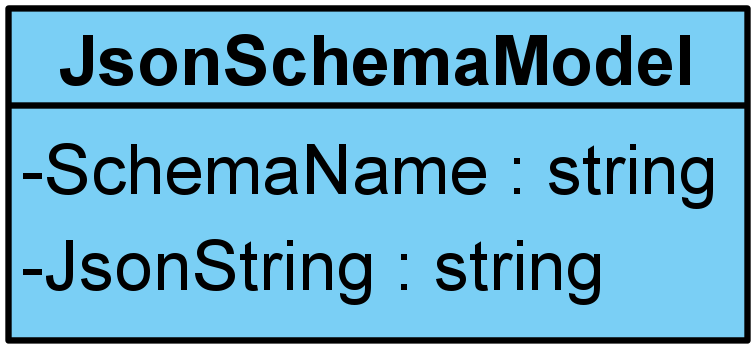
\includegraphics[scale=0.25]{Images/JsonSchemaModel.png}
    \caption{The model of the \texttt{JsonSchema} table.}
    \label{JsonSchemaModel}
\end{figure}
% WordRatio
\begin{figure}[H]
    \centering
    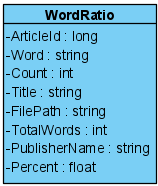
\includegraphics[scale=0.25]{Images/WordRatioModel.png}
    \caption{Diagram of WordRatioModel.}
    \label{WordRatioModel}
\end{figure}
\end{document}
